\documentclass[11pt,a4paper]{article}
\usepackage[margin=25mm]{geometry}
\usepackage[T1]{fontenc}
\usepackage{lmodern,microtype,amsmath,amssymb,amsthm}
\usepackage{booktabs,tabularx,longtable,array,enumitem,float}
\usepackage[numbers,sort&compress]{natbib}
\usepackage{xcolor,tikz}
\usetikzlibrary{arrows.meta,positioning,fit,backgrounds}
\usepackage[hidelinks]{hyperref}
\usepackage{url}
\urlstyle{same}
\setlength{\emergencystretch}{2em}
\setlength{\parskip}{3pt}
\setlist{nosep,leftmargin=*}
\newtheorem{proposition}{Proposition}
\newtheorem{definition}{Definition}
\newcommand{\oc}{OpenCorvus}
\newcommand{\src}{\texttt{bd2d6bd18eda}}
\newcommand{\pending}[1]{\textit{[Pending empirical evidence: #1]}}
\newcommand{\code}[1]{\texttt{\detokenize{#1}}}
\newcolumntype{Y}{>{\raggedright\arraybackslash}X}
\title{OpenCorvus: Separating Execution Ownership and Delivery Evidence in Long-Horizon Agent Work}
\author{Non-experimental working manuscript\\\small Author names and affiliations to be supplied}
\date{10 September 2026}
\begin{document}
\maketitle
\begin{abstract}
Long-horizon agent work can span multiple execution attempts, tools, participants, and process failures. A completed conversation is consequently an insufficient description of what ran, who retained authority to commit a transition, and which outputs informed delivery acceptance. This paper studies these distinctions in \oc{}, an open-source agent runtime. We develop an analytical model that separates business identity, execution occurrences, physical ownership, and revision-specific evidence. We map the model to a fixed source snapshot, focusing on fact reduction, transaction-scoped lease checks, and artifact read--selection--publication relations. Conditional propositions characterize stale-owner rejection within guarded database transitions, evidence-reference closure, and eventual rediscovery under explicit availability and fairness assumptions. Counterexamples delimit these properties: database fencing does not establish exactly-once external effects, complete reading does not establish semantic correctness, and final delivery does not establish dependency-order compliance. We provide a prospective evaluation protocol for fault recovery, independently accepted task outcomes, and mechanism costs. \pending{comparative outcomes, effect estimates, and any claim of practical improvement await experiments.} This manuscript reports a design analysis and protocol, not an empirical validation of the runtime.
\end{abstract}
\noindent\textbf{Keywords:} agent runtimes; execution identity; durable state; artifact provenance; recovery; software engineering.

\section{Introduction}
Large language model (LLM) agents combine generated decisions with tools and environmental feedback. Software agents make this interaction concrete: they inspect repositories, edit files, execute commands, and revise their work. SWE-agent studies interfaces for such interaction, while OpenHands provides an extensible platform for software-oriented agents \citep{sweagent,openhands}. These capabilities support workflows in which a single user objective outlives an individual model response or process. The resulting engineering problem concerns both useful reasoning and the continuity of accountable execution.

Consider a task that asks an agent to investigate a dataset, synthesize findings, and produce a reviewed report. A synthesizer may be restarted after a tool response is lost; a reviewer may consume an early revision; a final publisher may produce a well-formed document even when the intended review has not occurred. Three questions then have different answers: did a physical operation finish, did the correct execution occurrence receive its result, and does the deliverable satisfy the requested acceptance criteria? Treating these questions as one status obscures both failures and recovery decisions.

This distinction is motivated by retained \oc{} project records, rather than by a new experiment. A historical seven-role workflow produced a final report while the fact checker and report writer were created before the synthesizer reached terminal success. The retained audit also records an initial publication failure and a later publication path \citep{ocsource}. This case cannot establish the failure rate of the current system. It demonstrates why final output and process compliance require separate evidence. Section~\ref{sec:limits} explains the provenance and limitations of that record.

Durability itself is established territory. Temporal documents history-driven workflow progression, LangGraph persists graph checkpoints, and the OpenHands Software Agent software development kit (SDK) describes event-sourced conversation state and recovery \citep{temporal,langgraph,ohsdk}. Similarly, leases and causal ordering have a long history in distributed systems \citep{leases,lamport}. The research question is therefore narrower than whether agents should have persistent state:
\begin{quote}
How can a runtime represent the relationship between task acceptance, exact execution occurrences, physical ownership, and evidence revisions, and which correctness properties follow from that representation under stated assumptions?
\end{quote}

We study \oc{} as a concrete system at source snapshot \src{}, using source inspection and retained records. Our analytical contribution is a decomposition of this question into three inspectable boundaries: facts to control projection, ownership to guarded transitions, and observations to accepted delivery. We provide (i) an explicit semantic model, (ii) conditional propositions and counterexamples tied to selected implementation paths, and (iii) an evaluation protocol that distinguishes infrastructure continuity from task quality. These are contributions of the present manuscript. Whether the integrated design improves practical outcomes, and whether its combination warrants a stronger novelty claim, remain questions for comparison and measurement.

This scope has two consequences. First, we do not present event sourcing, leases, structured collaboration, or provenance as newly invented primitives. Second, a source-level argument is not a certification of the whole runtime. The analysis identifies implementation obligations and specifies experiments capable of falsifying stronger claims. No new model runs, fault injections, adoption studies, or comparative benchmark results are reported here.

\section{Background and Related Work}\label{sec:related}
\paragraph{Agent interfaces and collaboration.}
SWE-agent introduces an agent--computer interface with search, viewing, editing, and feedback facilities, and evaluates interface alternatives \citep{sweagent}. OpenHands combines a software execution environment with tools and delegation \citep{openhands}. AutoGen organizes applications through conversable agents and conversation programming \citep{autogen}. MetaGPT uses specialized roles, structured outputs, and publish--subscribe communication within standard operating procedures \citep{metagpt}. These studies motivate attention to interaction and handoff design. We do not infer the absence of recovery or provenance facilities in their current code from the emphasis of a particular paper version.

\paragraph{Runtime state and durable execution.}
The OpenHands Software Agent SDK is especially close prior work. Its versioned paper describes immutable agent configuration, an append-only event log, mutable conversation metadata, and reconstruction of conversations from persisted state \citep{ohsdk}. It also separates action, execution, and observation. Any claim that \oc{} first makes agent execution event-based or recoverable would therefore be unsupported. AIOS studies an agent operating-system abstraction with centralized system-call scheduling and context management \citep{aios}. These mechanisms operate at different boundaries from a task acceptance decision, but their existence rules out framing resource scheduling as a new idea.

LangGraph's version-pinned persistence documentation describes checkpoints at graph super-steps, identified by threads, with persisted state available across runs \citep{langgraph}. Temporal's History Service documentation relates history updates, mutable state, timer tasks, and transfer tasks \citep{temporal}. We cite these as technical documentation, not peer-reviewed empirical results. They are direct precedents for separating durable execution state from physical work delivery. A future baseline must be selected from a specified implementation with matched capabilities; mentioning a system here does not establish experimental comparability.

\paragraph{Ownership and provenance.}
Lamport formalizes causal precedence as a partial order \citep{lamport}; the presence of increasing timestamps alone does not establish the dependency relation of an application. Gray and Cheriton analyze leases with explicit failure and clock assumptions \citep{leases}. We reuse the idea of bounded authority and examine the more limited transaction boundary actually visible in \oc{}. The World Wide Web Consortium (W3C) PROV data model separates entities, activities, agents, and derivation relations \citep{prov}. Our artifact model draws a conceptual parallel to these distinctions; we do not claim that \oc{} implements the PROV standard or validates its constraints.

\paragraph{Evaluation of extended work.}
SWE-EVO constructs software evolution tasks from release histories and validates behavior using before/after execution \citep{sweevo}. It is a candidate workload source because evolving requirements can involve multiple changes. Its task validation does not by itself observe execution ownership or crash recovery. Consequently, our protocol separates controlled infrastructure faults from task acceptance, and treats task selection and oracle coverage as explicit validity concerns. We have not run SWE-EVO in this study.

Table~\ref{tab:related} summarizes the role of these sources in our argument. It is a comparison of documented focus, not a feature-absence leaderboard or an exhaustive literature review. The audited versions and reading scope are recorded in the accompanying citation notes.
\begin{table}[htbp]
\centering\small
\begin{tabularx}{\linewidth}{@{}lYY@{}}
\toprule
Source family & Documented focus used here & Implication for this study \\
\midrule
SWE-agent; OpenHands & Tool interfaces and software execution & Hold tool access constant in comparisons. \\
AutoGen; MetaGPT & Conversation and role-based collaboration & Do not claim structured handoffs are new. \\
OpenHands SDK; AIOS & Runtime state, lifecycle, or resource handling & Compare semantic boundaries, not platform size. \\
LangGraph; Temporal & Persisted workflow progression & Treat durable execution as prior art. \\
Leases; PROV & Bounded authority and provenance relations & State assumptions and semantic limits. \\
SWE-EVO & Executable software evolution tasks & Add recovery and lineage oracles separately. \\
\bottomrule
\end{tabularx}
\caption{Prior work constrains the claims and evaluation design. Each row refers to the versions cited in the text.}\label{tab:related}
\end{table}

\section{Problem Formulation}\label{sec:model}
\subsection{Objects and research unit}
We use \emph{long-horizon work} to describe work whose acceptance depends on several causally related interactions, revisions, or execution occurrences, with possible interruption between them. Wall-clock duration, token consumption, or the number of agents alone is not a definition of difficulty. A workload should report dependency depth, revision count, tool interactions, and fault exposure separately.

Let a project be an isolation context $p$. A task $\tau$ is a persistent business identity within that context. An epoch $e$ distinguishes lifecycle intervals when a task is reopened. A delivery requirement is represented by a slice revision $s$; revising a requirement produces a distinct reference rather than silently changing the meaning of an earlier acceptance. A session groups conversational state, while a turn identifies a particular unit of agent execution within that session. An occurrence $o$ identifies one execution instance under the relevant task, epoch, and dispatch identity. These are analytical categories: their concrete identifiers occupy different source structures rather than one universal tuple.

An external effect $x$ is a tool-visible operation such as a filesystem write or a service request. Its real-world outcome may become known before, after, or never through a durable observation. An artifact reference $a=(p,\tau,i,r,h)$ denotes context, identity, revision, and payload digest. This is a normalized notation, not the literal wire format: some implementation locators carry project and task authority through their enclosing scope, and resource locators additionally include snapshot, path, media type, and length. A digest binds bytes under an integrity assumption; it is not a truth certificate.

\begin{table}[htbp]
\centering\small
\begin{tabularx}{\linewidth}{@{}lYY@{}}
\toprule
Symbol & Meaning & Must not be inferred solely from it \\
\midrule
$\tau,e$ & Task identity and lifecycle epoch & A particular physical execution \\
$o$ & Exact execution occurrence & Every run sharing its session \\
$\ell$ & Lease for a target and owner & Permission for all external effects \\
$a$ & Exact artifact reference & Correctness or relevance of its contents \\
$q$ & Observation with scope and lineage & Acceptance of all requirements \\
$d$ & Acceptance decision over revisions & Independent validation of that judgment \\
\bottomrule
\end{tabularx}
\caption{Distinct identities support distinct forms of evidence.}\label{tab:objects}
\end{table}

\subsection{State and transition model}
Let $F_{\leq k}$ be a durable fact prefix under a specified consistent database view. Let $C_k$ be configuration and policy, and $L_k$ the lease records visible in that view. We write
\begin{equation}\label{eq:projection}
P_{k,t}=R(F_{\leq k},C_k,L_k,t).
\end{equation}
Here $R$ abstracts the relevant implementation reducers; it is not a claim that the repository contains one function with this signature. The time parameter $t$ supports expiry and deadline classification. Durable facts and mutable ownership metadata are explicitly separate. In particular, lease expiry fields are updated by renewal and release. We do not model every runtime variable as immutable.

A hint $h$ requests that the runtime inspect durable state. A hint is not an acceptance fact or an authority grant. A scan computes a projection and may activate eligible work, record a bounded failure, or arrange a later wake. The local driver's revision counter coalesces requests arriving during an owned scan. A periodic enumeration of live tasks provides a second opportunity to discover durable work after a hint is lost. These mechanisms concern control progress; the LLM still chooses domain actions subject to available tools and authorization.

For a target $u$, define $\mathrm{cur}(L,u)$ as the record selected by the implementation's current-lease rule. A lease $\ell$ is valid for owner $o$ at an assertion instant $t$ when
\begin{equation}\label{eq:lease}
V(\ell,o,u,t) \iff \ell=\mathrm{cur}(L,u)\ \land\ \ell.\mathrm{owner}=o\ \land\ t<\ell.\mathrm{expiry}.
\end{equation}
The rule includes exact lease identity. A worker's remembered expiry does not replace a fresh assertion. The current implementation orders lease rows by activation time and identity; that ordering must be consistent with acquisition order for the intended replacement semantics.

\subsection{Evidence and acceptance}
Write $\mathrm{Read}(o,a)$ when recorded read windows fully cover the bytes of the exact reference $a$ in the required action scope. Write $\mathrm{Select}(o,a)$ when the same scoped evidence is explicitly selected for use. For an output $b$, let $\mathrm{Sources}(b)$ be its declared source references. A minimal publication condition is
\begin{equation}\label{eq:evidence}
\forall a\in\mathrm{Sources}(b):\quad \mathrm{Read}(o,a)\land\mathrm{Select}(o,a).
\end{equation}
This condition is about declared references. If the declared set is empty, it holds vacuously. It does not prove that all substantively necessary sources were declared, that the producer understood them, or that $b$ follows from them.

An acceptance decision $d$ binds a task, its relevant lifecycle boundary, selected deliverable references, evidence references, and accepted requirement revisions. We distinguish the runtime's recorded acceptance, $A_{\mathrm{run}}(d)$, from an independent task oracle $A_{\mathrm{ext}}(\tau,b)$. The first establishes what the runtime recorded and attributed. The second tests whether the requested outcome is actually satisfied. The evaluation reports them separately and does not define success using the runtime decision alone.

For a declared dependency graph $G=(N,E)$, a strict dependency condition would require the relevant predecessor occurrence to complete successfully before a dependent dispatch is admitted. This is stronger than reference closure and stronger than eventually collecting all outputs. In the inspected architecture, the orchestrator is responsible for following declared workflow dependencies; the host does not universally enforce that graph as a scheduling frontier. We therefore treat dependency compliance as an observed property to evaluate, not an invariant provided by the runtime.

\subsection{Failure model and assumptions}\label{sec:assumptions}
The analytical model permits process crashes, lost or repeated hints, delayed results, interrupted model streams, tool timeouts, and a worker continuing after its ownership has expired. It also permits external operations whose outcome is unknown locally. The following assumptions delimit the propositions:
\begin{enumerate}[label=A\arabic*.]
\item Guarded database operations use transactions with the isolation required to serialize competing ownership changes and assertions, and committed records survive the considered crashes.
\item A protected transition checks the exact target, owner, and lease in the same transaction as the transition. A lease supersession requires valid domain authority. Unguarded transitions are outside this proposition.
\item Lease time observations and row ordering are consistent with the intended acquisition/expiry order. Arbitrary backward clock jumps, inconsistent cross-host clocks, and storage corruption are outside the guarantee. Actual deployments must characterize these assumptions.
\item Artifact storage retains the referenced version; canonical reads and digests identify its bytes correctly; the scoped read/selection collectors are faithful to actual tool outcomes. Malicious storage and digest collisions are excluded from the byte-integrity argument.
\item For eventual rediscovery, the database becomes readable, the driver remains live, enumeration repeatedly includes unresolved tasks, timers eventually run, and capacity admission is fair. An operator-gated state additionally requires the relevant operator action.
\end{enumerate}
The model provides neither Byzantine fault tolerance nor a claim that arbitrary model decisions satisfy the task. It does not assume atomic commitment across a database and an arbitrary external service. Those exclusions are essential to interpreting recovery behavior.

\section{Runtime Design}\label{sec:design}
\subsection{Facts, projections, and physical activation}
Figure~\ref{fig:architecture} shows the separation used in our analysis. Domain inputs and observed outcomes contribute durable facts. Reducers interpret those facts with lifecycle policy, ownership, and time. The driver requests scans and arranges activation; a scan is not itself a new task definition. Agent turns produce real tool requests and observations, and delivery decisions refer back to identifiable evidence.

\begin{figure}[htbp]\centering
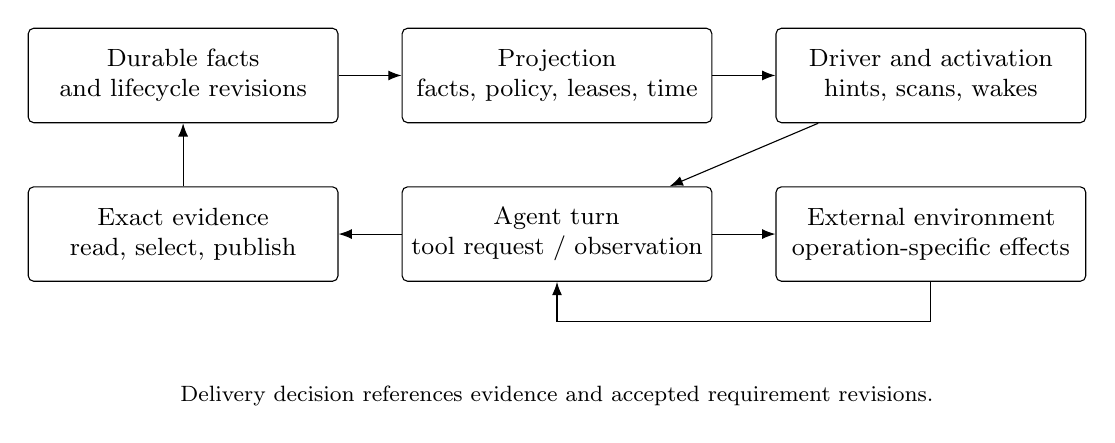
\begin{tikzpicture}[font=\small,>=Latex,box/.style={draw,rounded corners=2pt,align=center,minimum height=12mm,text width=37mm},node distance=8mm]
\node[box] (facts) {Durable facts\\and lifecycle revisions};
\node[box,right=of facts] (reduce) {Projection\\facts, policy, leases, time};
\node[box,right=of reduce] (driver) {Driver and activation\\hints, scans, wakes};
\node[box,below=of facts] (evidence) {Exact evidence\\read, select, publish};
\node[box,below=of reduce] (turn) {Agent turn\\tool request / observation};
\node[box,below=of driver] (world) {External environment\\operation-specific effects};
\draw[->] (facts)--(reduce);\draw[->] (reduce)--(driver);
\draw[->] (driver)--(turn);\draw[->] (turn)--(world);
\draw[->] (turn)--(evidence);\draw[->] (evidence)--(facts);
\draw[->] (world.south) -- ++(0,-5mm) -| (turn.south);
\node[align=center,font=\footnotesize,below=12mm of turn] {Delivery decision references evidence and accepted requirement revisions.};
\end{tikzpicture}

\caption{Analytical view of selected \oc{} paths. Arrows denote information or authority dependencies, not a claim of a single atomic pipeline. External effects cross the database boundary.}\label{fig:architecture}
\end{figure}

The root-ingress reducer illustrates the distinction between a pending request and permission to continue it. In the inspected source, operator abandonment and integrity faults are classified explicitly; lifecycle epochs can make older ingress inapplicable; validated decisions can resolve it; and live leases identify an already-owned activation. These alternatives matter because blindly re-running a queued instruction after a restart can apply it to a different lifecycle interval. The reducer and wake classifier expose whether progress depends on a deadline, an infrastructure fact, or operator input. A host fault is not evidence that a domain task was successfully completed.

The driver addresses a separate problem: durable work may exist without a surviving in-memory notification. When a request arrives, the local task entry's revision increases. An existing scan owner absorbs the notification; otherwise the driver attempts capacity admission. The owner scans for a bounded number of passes, records requested wake instants, and rechecks when revisions change. Faults and non-progress are paced with backoff. The periodic live-task enumeration retains rejected admissions in its current page rather than committing past them. This mechanism supplies rediscovery opportunities without making local notification counts the business state.

The schematic procedure below is an abstraction of these selected paths. It deliberately omits policy-specific reducer branches, retry coefficients, and project entry-point wiring. It is not an executable replacement for the runtime.
\begin{quote}\small
\begin{enumerate}
\item On a hint for task $\tau$, increment its local revision. Coalesce with a running owner or request a scan slot.
\item Under an admitted owner, read the current fact revision and invoke the scan against durable state.
\item Collect activation and wake information. If new input arrived, rescan within the pass budget; otherwise stop the pass loop.
\item On a bounded failure or lack of progress, retain the condition and arrange a later attempt under backoff.
\item Release local scan ownership and arm the earliest retained wake, if any.
\item Independently enumerate live tasks. Keep capacity-rejected entries eligible for later admission.
\end{enumerate}
\end{quote}

Local scan ownership and database activation leases serve different purposes. The former avoids redundant work within a driver instance; the latter guards selected durable transitions across physical contenders. Neither substitutes for project-scoped data access or for exact execution lineage. A complete deployment audit would need to trace every production entry point and ownership boundary; this paper does not claim to have formally verified that entire surface.

\subsection{Ownership checked at the durable transition}
The lease module represents a target, an owner occurrence, a lease identity, activation time, and expiry. Acquisition reads the current lease in a transaction and normally refuses a new contender while that lease is unexpired. Explicit supersession is a separate authority-bearing case. Renewal requires the current identity and owner, updates the expected expiry, and appends a grant record. Release expires the exact current lease. Thus the durable structure includes both mutable expiry and grant history.

A stale worker is rejected only where a protected transition actually rechecks ownership. For example, the dispatch-lineage commitment path accepts an admission owner, asserts its lease when present, requires a durable descriptor for the exact dispatch turn, and consumes the admission in the same transaction. The optional admission parameter is material: this code inspection does not imply that every invocation carries an admission lease. Likewise, task-completion closure uses a lifecycle-scoped target and translates failed ownership assertions into an explicit closure conflict.

Figure~\ref{fig:recovery} separates database rejection from an external effect's outcome. If a worker performs an external operation before it loses its lease, a later database rejection cannot erase that operation. If an acknowledgement is lost, the runtime may know that it lacks a result while the external service has already committed the effect. Safe recovery requires an operation-specific reconciliation or idempotency contract; the existence of a lease is insufficient.

\begin{figure}[htbp]\centering
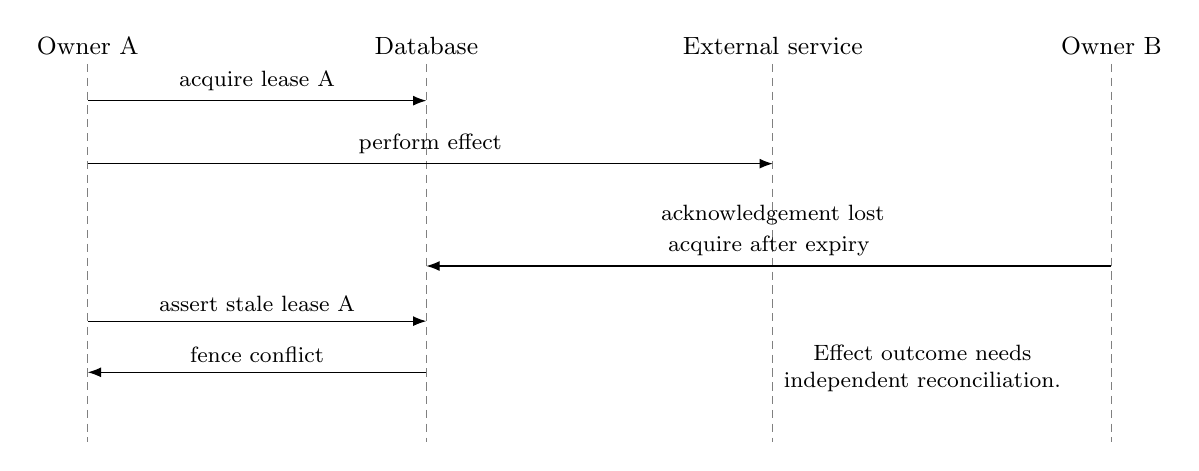
\begin{tikzpicture}[font=\small,>=Latex]
\node (old) at (0,0) {Owner A};\node (db) at (4.3,0) {Database};\node (ext) at (8.7,0) {External service};\node (new) at (13,0) {Owner B};
\foreach \n in {old,db,ext,new} {\draw[densely dashed,gray] (\n.south)--++(0,-48mm);}
\draw[->] (0,-.7)--node[above,font=\footnotesize]{acquire lease A}(4.3,-.7);
\draw[->] (0,-1.5)--node[above,font=\footnotesize]{perform effect}(8.7,-1.5);
\node[font=\footnotesize,align=center] at (8.7,-2.15) {acknowledgement lost};
\draw[->] (13,-2.8)--node[above,font=\footnotesize]{acquire after expiry}(4.3,-2.8);
\draw[->] (0,-3.5)--node[above,font=\footnotesize]{assert stale lease A}(4.3,-3.5);
\draw[->] (4.3,-4.15)--node[above,font=\footnotesize]{fence conflict}(0,-4.15);
\node[font=\footnotesize,align=center] at (10.6,-4.1) {Effect outcome needs\\independent reconciliation.};
\end{tikzpicture}

\caption{Schematic failure sequence, not an observed experimental trace. The stale owner's guarded database write is rejected; whether its earlier external effect occurred requires separate evidence.}\label{fig:recovery}
\end{figure}

\subsection{Evidence is read, selected, and published}
The artifact catalog provides exact references to engine artifact revisions, task snapshots, and resources. The read path checks identity and integrity rather than interpreting an unversioned name as the latest content. Text may be read in bounded windows. The recorded windows must collectively cover the exact reference before it qualifies as a complete read in the relevant scope. A complete transport record means that the bytes were delivered through that interface; it does not reveal how a model attended to them.

The publication function accepts observed and selected locator sets from its host caller. Every declared source locator must belong to both sets. Resource checks also relate the publication to its task and validate referenced resource content. The two inspected public call paths supply these sets differently: the native tool derives scoped read and selection facts preceding the current publication, whereas the plugin host tracks reads and selections within the invocation. Both call the same catalog publication function. The authority of the input sets depends on those collectors; the function cannot prove their origin merely from a supplied array.

Figure~\ref{fig:evidence} illustrates the resulting relation. Exact references prevent a reviewer from silently being credited with a later revision. Explicit selection records a producer's declared use. Yet neither guarantees comprehensive citation: a producer can omit a relevant source or misunderstand one. Domain review and independent acceptance remain separate activities.

\begin{figure}[htbp]\centering
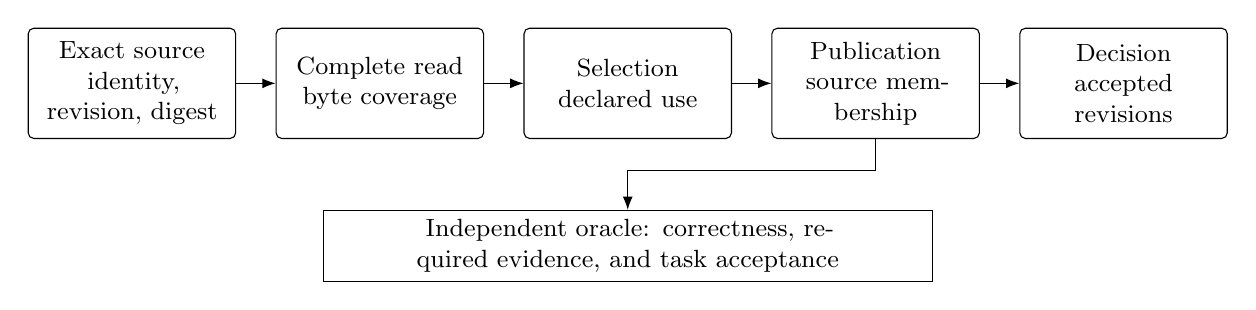
\begin{tikzpicture}[font=\small,>=Latex,box/.style={draw,rounded corners=2pt,align=center,text width=24mm,minimum height=14mm},node distance=5mm]
\node[box] (ref) {Exact source\\identity, revision, digest};
\node[box,right=of ref] (read) {Complete read\\byte coverage};
\node[box,right=of read] (select) {Selection\\declared use};
\node[box,right=of select] (pub) {Publication\\source membership};
\node[box,right=of pub] (accept) {Decision\\accepted revisions};
\draw[->] (ref)--(read);\draw[->] (read)--(select);\draw[->] (select)--(pub);\draw[->] (pub)--(accept);
\node[draw,align=center,below=9mm of select,text width=75mm] (oracle) {Independent oracle: correctness, required evidence, and task acceptance};
\draw[->] (pub.south) -- ++(0,-4mm) -| (oracle.north);
\end{tikzpicture}

\caption{Evidence path for one declared source. Byte coverage, declared use, publication, and acceptance have different semantics. The independent oracle evaluates the deliverable separately.}\label{fig:evidence}
\end{figure}

\subsection{Delivery decisions and responsibility}
The inspected completion-decision schema records orchestrator session/message identity, tool call/part identity, evidence locators, deliverable locators, accepted slice revision identifiers, workflow binding, and recording time. It includes host-derived references to outputs from terminal workflow nodes. A reader locates the decision for an exact task and terminal time. This makes an acceptance decision inspectable as a particular act with referenced material.

The closure establishes a recorded set and attribution, not a proof that the model judged correctly. An output from a terminal workflow node does not certify that all preceding nodes executed in order. A passing host checker certifies only the tested contract and observed execution context. Visual or domain judgments need their own evidence; tests over unrelated code or a final status label cannot replace them. This boundary permits meaningful accounting when the runtime records completion but an independent evaluator rejects the deliverable.

\section{Implementation and Audit Scope}\label{sec:implementation}
The source inspection is fixed to commit \code{bd2d6bd18eda05f35326adc231289e56d0a2dfcf}. The manuscript is stored in a later documentation-only state. Product source is not modified for this paper. Table~\ref{tab:implementation} provides the principal source anchors; the accompanying source map records symbols, line spans, and pre-existing claim identifiers. The symbols are preferable to floating line numbers when a reader inspects another revision.

\begin{table}[htbp]\centering\small
\begin{tabularx}{\linewidth}{@{}YY@{}}
\toprule
Module under \code{packages/opencorvus/src/} & Inspected responsibility \\
\midrule
\path{engine/task-root-ingress-reducer.ts} & Classify ingress facts and wake conditions. \\
\path{engine/task-control-driver.ts} & Coalesce hints, admit scans, retain wakes, enumerate live tasks. \\
\path{engine/control-lease.ts} & Acquire, assert, renew, and release exact ownership. \\
\path{engine/dispatch-lineage.ts} & Bind dispatch to a durable turn descriptor; guarded admission consumption. \\
\path{engine/task-completion-closure.ts} & Lifecycle-scoped ownership of completion closure. \\
\path{engine/completion-decision-facts.ts} & Typed acceptance references and terminal-time lookup. \\
\path{artifact-catalog/index.ts} & Exact reads, resource integrity, source membership at publication. \\
\path{agent/artifact-provenance-facts.ts} & Scoped complete reads and selected source facts. \\
\path{tool/artifact-catalog.ts}; \path{tool/plugin-tool-host.ts} & Supply provenance from actual tool/action scope. \\
\bottomrule
\end{tabularx}
\caption{Inspected implementation anchors. This table reports source responsibilities, not runtime benchmark validation.}\label{tab:implementation}
\end{table}

The repository uses TypeScript and database access through its storage abstraction; the lease acquisition wrapper uses an immediate transaction. These are implementation choices rather than prerequisites of the semantic model. The model requires an appropriate transactional boundary and persistent identity, not a particular programming language. Existing architecture documents describe capabilities and package projection, but this manuscript does not count packages, agents, providers, or tools as research contributions. Live provider projection, all production entry points, and full cross-project isolation have not been exercised for this study.

We preserve the repository's earlier evidence package as historical input. Its machine claim matrix remains the original claim authority; the new source map relates paper passages to that package and to inspected source. It does not upgrade old implementation statuses or acceptance receipts. Source inspection can establish that a check exists in a selected path. Establishing that all actual runs traverse the intended checks requires additional execution and coverage evidence.

\section{Conditional Properties and Counterexamples}\label{sec:properties}
The following propositions are elementary consequences of the abstract contracts and their stated assumptions. They delimit claims about the design; they are not novel distributed algorithms, machine-checked proofs, or a whole-program verification of \oc{}.

\begin{proposition}[Stale identity at a guarded transition]\label{prop:fence}
Under A1--A3, after a replacement lease becomes current for target $u$, a transaction asserting a different lease identity for $u$ cannot successfully perform a transition guarded by that assertion.
\end{proposition}
\begin{proof}
Consider the serial position of the protected transaction after the replacement transaction. A1 makes the replacement visible in its consistent view. Under A3 the current-lease rule selects the replacement. The exact-identity conjunct in Equation~\ref{eq:lease} is therefore false for the older identity. A2 places assertion and transition in the same transaction, so the failed assertion prevents that guarded transition. A transaction serialized before replacement is outside the stated temporal case.\end{proof}

This statement does not assert that the lease remains unexpired at physical commit time after an earlier check; it concerns the check's serialized view. It also does not prove that unguarded operations, arbitrary plugin actions, or external services observe the lease. The conditional guarantee must be instantiated for each protected path. A clock anomaly that changes which row is current invalidates A3 and requires a deployment-specific analysis.

\begin{proposition}[Declared-source reference closure]\label{prop:closure}
Assume A4 and that a publication reaches the inspected membership checks with faithful observed and selected locator sets. If the publication is accepted through those checks, every declared source has a complete read and selection in the caller's required scope.
\end{proposition}
\begin{proof}
Suppose an accepted publication declared a source $a$ without a complete scoped read or without a selection. Faithful collectors would omit $a$ from at least one supplied set. The publication loop checks membership in both sets for each declared locator and raises an error on either failure. The assumed acceptance therefore contradicts the corresponding membership check. Exact locator equality and A4 keep this argument tied to the same revision.\end{proof}

The proposition is intentionally limited to declared sources. Consider a report requiring evidence from documents $a_1$ and $a_2$. A producer may read and select $a_1$, omit $a_2$, and publish a plausible but unsupported conclusion. Equation~\ref{eq:evidence} still holds. Even declaring and reading both documents would not prove the inference valid. The oracle must therefore inspect substantive evidence coverage and reasoning separately from transport closure.

\begin{proposition}[Eventual opportunity for rediscovery]\label{prop:discovery}
Under A5, an unresolved task that remains eligible and repeatedly appears in the live-task enumeration eventually receives an admitted scan, even if its original hint was lost.
\end{proposition}
\begin{proof}
Repeated enumeration provides further admission requests independently of the original hint. Capacity-rejected entries remain eligible for subsequent requests. Fair admission in A5 gives an admission after finitely many such opportunities. A live driver and eventually readable storage allow the scan to occur. Without fair admission or continued inclusion in the enumeration, this conclusion does not follow.\end{proof}

An admitted scan is not task completion. It may correctly identify an operator-gated condition, produce another bounded failure, or dispatch an agent that makes no useful progress. Neither the proof nor the implementation inspection gives a latency bound. A bound would additionally require quantitative limits on enumeration, backoff, admission, storage response, and scan duration. This is why the evaluation measures discovery, recovery, and acceptance separately.

\subsection{External effects and indistinguishable local states}\label{sec:effects}
Consider two executions of an external operation $x$. In execution $H_1$, the service commits $x$ and the acknowledgement is lost before a local observation is durable. In execution $H_2$, the request never commits and the same local observation is absent. If the only available durable local facts are identical, a recovery algorithm using those facts alone cannot distinguish $H_1$ from $H_2$. Retrying may duplicate $x$ in $H_1$; refusing to retry may leave $x$ undone in $H_2$.

Consequently, an exactly-once claim for an arbitrary external effect requires information beyond local lease checks: for example, a service-supported idempotency key and queryable result, a shared transaction, or a domain-specific reconciliation procedure. We do not assert that \oc{} supplies these for every tool. The protocol records the distinct states ``confirmed committed'', ``confirmed not committed'', and ``unknown'', and inspects the external operation independently. Local idempotent artifact publication does not resolve this general ambiguity.

\subsection{Completion and causal compliance}
A second counterexample separates output closure from dependency compliance. Let a workflow require $n_1\rightarrow n_2$, where $n_2$ must review the accepted result of $n_1$. If $n_2$ starts on an early artifact and $n_1$ later publishes a final revision, a task may eventually contain both outputs. A final decision referring to an output set does not retroactively establish that $n_2$ consumed the final predecessor result. The dependency property needs exact occurrence and artifact-revision relations, not only timestamps or node names.

The historical seven-role record is compatible with this distinction, but the counterexample is a logical construction and does not depend on estimating a failure probability from that record. In future execution traces, a dependency oracle must compare predecessor success, dependent dispatch, and consumed references. When cross-process order cannot be established by lineage or a common sequencer, the event order is reported as unresolved rather than inferred from unsynchronized clocks.

\subsection{What these properties leave open}
The propositions do not establish global linearizability, arbitrary-process isolation, complete application-level idempotency, or semantic task success. Their practical value is to expose obligations that can be checked: transaction placement, exact identity, scoped read collectors, live-task coverage, and external effect oracles. If an obligation fails, an implementation-level claim must be narrowed or the implementation investigated. The analysis does not reinterpret a failing run as a success because another layer happened to produce a deliverable.

\section{Experimental Design}\label{sec:evaluation}
The evaluation targets four questions: whether specialization improves professional task quality; whether retained updates improve unseen work; whether any gains justify total resources and human effort; and whether improvement preserves previously useful capabilities. This manuscript contains the method and experimental design; performance measurements are not yet reported.

\paragraph{Task families and partitions.}
The primary family is evidence-based analytical reporting: each task provides a fixed source bundle, a computational question, and a deliverable contract. Acceptance requires reproducible calculations, support for load-bearing claims, and agreement between the rendered report and canonical results. A second family uses software maintenance tasks with executable functional checks and exact repository snapshots. Enrollment requires at least three dependent stages, an intermediate artifact consumed and checked in a later stage, and an independently checkable final deliverable. These requirements apply to the task contract, not the number of agents. We record required stages, tool interactions, and input resource size. The reuse horizon $T$ counts subsequent assignments to the retained organization; it does not assert a particular single-task duration or context length.

Tasks are partitioned by source provenance or repository, before development, into update tasks, unseen future tasks from the same family, and a retained-capability test set. Reworded questions over the same evidence and related issues from one repository remain in the same partition. A separate, untouched family tests cross-domain transfer only when its tools and contracts are already compatible with the starting package; results from this setting are reported separately from within-domain generalization. Figure~\ref{fig:evolution} specifies the information boundary.

\begin{figure}[!t]
\centering
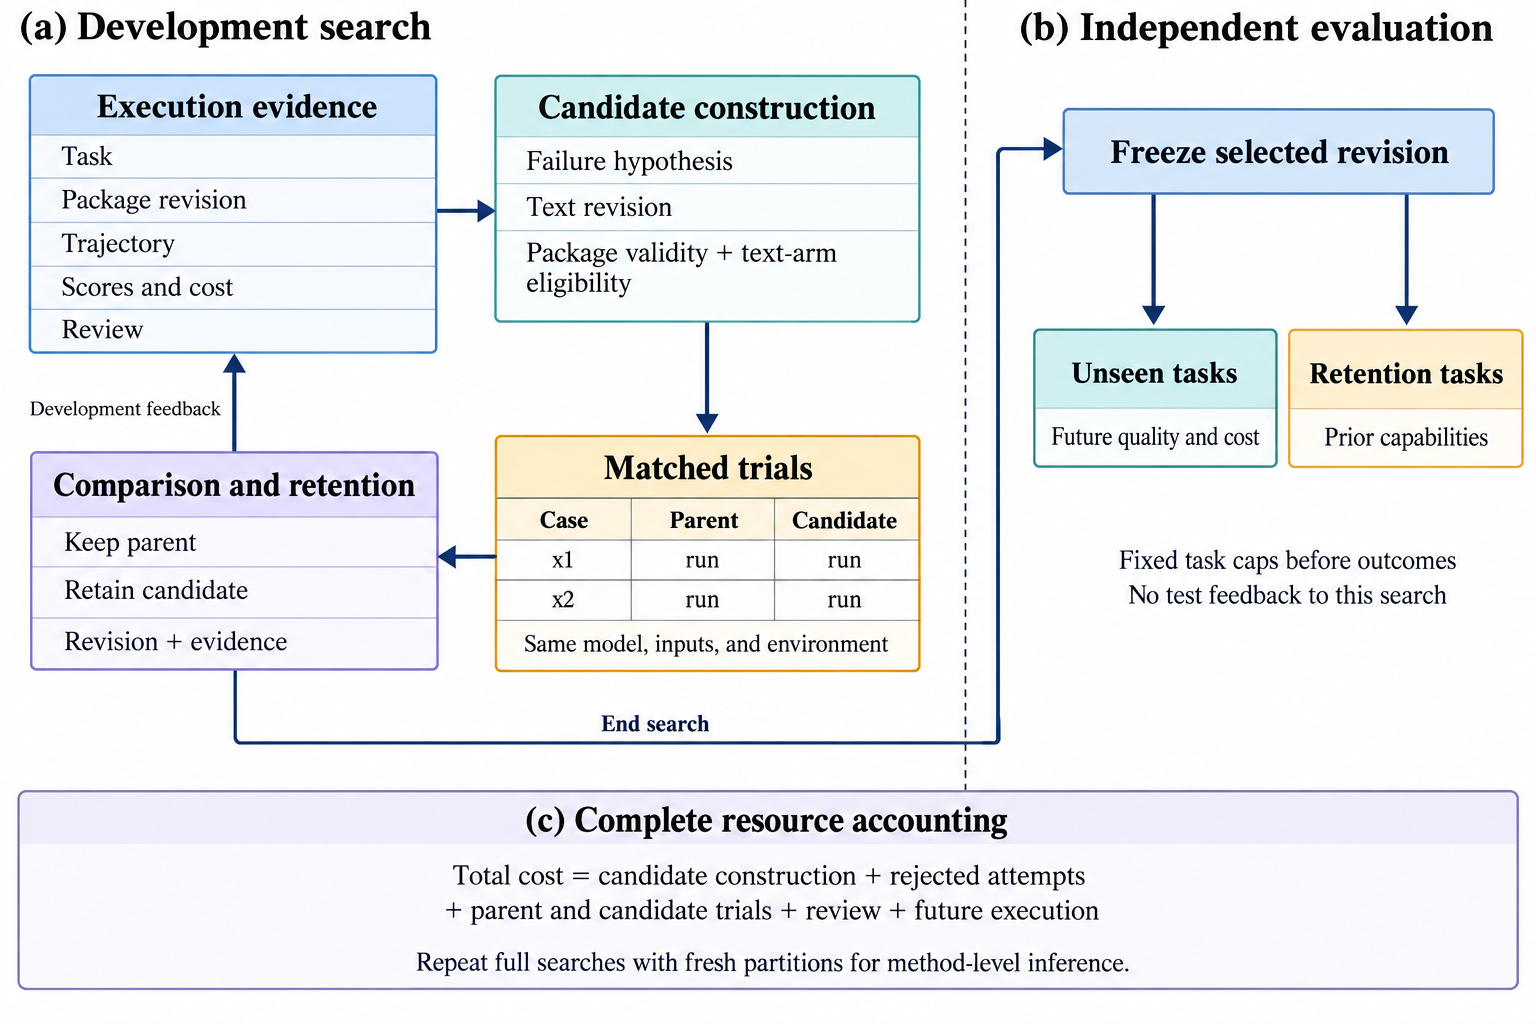
\includegraphics[width=\linewidth]{figures/evolution.png}
\caption{Organizational development and independent evaluation. Development trials supply evidence for candidate construction and retention. The final selected organization is frozen before independent unseen-task and prior-capability evaluation. The pairing matrix denotes trial slots, not measured results. Total resource accounting includes failed search attempts. A new search episode uses fresh partitions; test outcomes do not return to the same search.}
\label{fig:evolution}
\end{figure}


\paragraph{Controlled comparisons.}
All arms use the same foundation model, inference configuration, domain input access, and total resource ceiling. Table~\ref{tab:arms} defines successive organizational changes. For the collaboration contrast, one frozen generic instruction set supplies both the single agent and the fixed team with identical planning, execution, and checking procedures. The single agent receives the complete set, can use the union of the team's tools, and performs the same responsibilities within one iterative context. The team distributes those procedures to their corresponding roles; only participant addressing and the messages needed for delegation change. This contrast estimates the effect of distributing the same procedural knowledge across communicating agents, including its context and coordination costs. Neither arm is restricted to a one-shot response.

The fixed generic and specialized teams share the same role roster, workflow declarations, and capability allocations. Specialization changes the domain procedures, reference bindings, and output-contract instructions. The task's acceptance rubric and underlying source access remain identical. Each family's concrete instruction sets and deployment mappings are frozen before development, so a stronger manually authored baseline cannot be introduced after seeing test outcomes.

\begin{table}[!htb]
\centering\small
\begin{tabularx}{\linewidth}{@{}lYYY@{}}
\toprule
Arm & Organization & Domain procedures & Retained updates \\
\midrule
Single agent & One iterative tool-using agent & Complete generic instruction set & None \\
Fixed team & Generic expert roles & Same generic set, assigned by role & None \\
Specialized team & Fixed domain organization & Explicit procedures and contracts & None \\
EEO--text & Same initial specialized team & Same initial package & Experience-driven text revision \\
\bottomrule
\end{tabularx}
\caption{Primary comparisons. EEO--text follows the released text-authoring policy, with an additional research eligibility check on each realized diff. Structural search requires a separate generator and study arm.}
\label{tab:arms}
\end{table}

Search costs are charged before future execution. Each arm receives the same episode-wide ceiling $B$ over the same number of assigned future tasks. Before inspecting any test outcome, each arm allocates its post-search remainder to fixed per-task caps whose sum does not exceed that remainder. An arm with no search can allocate larger inference caps. Caps are not recycled across test tasks, and each execution starts from its prescribed isolated workspace. This prevents a costly early task from reducing a later task's allowance. Unfinished assigned tasks remain in the quality denominator. A supplementary comparison fixes per-task inference cost to expose the mechanism's effect without amortization; it is labeled separately and reports search overhead.

\paragraph{Optimizer control.}
The protocol compares EEO--text with a GEPA-based adaptation on the same initial package, eligible text surface, feedback access, model, and total budget \citep{gepa}. GEPA's execution modules are LLM components with inputs, outputs, and trajectories; package files are their editable parameters, not execution modules. An orchestrator or expert can consume several files, and a shared skill can influence several experts.

Before execution, the adapter must freeze a mapping from every eligible file and descriptive manifest field to its consuming modules and visible execution evidence. It must specify the feedback attached to shared resources, the update policy for a resource used by multiple modules, and how a parameter update reconstructs one complete candidate package. Shared content has one canonical value; it is not independently rewritten into conflicting role-specific copies. Both optimizers start from the same development inputs and pre-existing evidence, with identical feedback interfaces and visible fields. Each receives and pays for the observations generated by its own candidate trials; the methods do not exchange search trajectories. Integrity checks and held-out tests are identical.

The adaptation preserves GEPA's candidate pool and ancestry, Pareto-based candidate sampling, declared module-selection policy, and minibatch evaluation before broader development-set scoring. The reference version, reflection prompt, sampling sizes, selection policy, optional merge setting, and stopping rule are recorded with the file-to-module mapping. All adaptation, sampling, reflection, and evaluation costs count toward the same total ceiling; GEPA's rollout count is reported separately from that full accounting. The adapter and its configuration require implementation and freezing before this comparison can run. This control tests revision-policy value on a common substrate.

\paragraph{Outcomes and scoring.}
The primary outcome is binary contract satisfaction at the task level. Reporting tasks require computational checks and blinded review against a frozen rubric; software tasks require the prescribed functional checker. An LLM judge is supplementary and uses a separately fixed prompt and model. We report inter-reviewer agreement, adjudication rules, and task-level disagreement counts. Secondary outcomes are component quality, all model and tool consumption, elapsed time, intervention count and minutes, completion rate, and retention-set quality. Missing measurements, infrastructure failures, agent failures, and budget exhaustion receive explicit categories. Agent failure and budget exhaustion count as unsuccessful assigned tasks; infrastructure exclusions follow a rule fixed before arm outcomes are inspected.

\paragraph{Mechanism studies.}
The attribution ablation supplies both authors with identical raw run evidence, scores, and evaluator feedback. Both arms compute the analyst's structured hypothesis $H$ and charge its cost; only the treatment author receives $H$. Candidate-author calls and trial budgets are matched. This isolates the additional attribution message from access to the original evidence. A second ablation removes reusable domain references while preserving role instructions and tools. These tests distinguish the value of experience and resource packaging from generic extra inference. Role, dependency, and capability-allocation changes require separate structural-search arms. The EEO--text arm checks each realized candidate diff against the text space in Section~\ref{sec:evolution}: only eligible text resources, enumerated descriptive manifest fields, and the version label may change. Roles, dependencies, capability allocations, resource paths, and other manifest declarations remain fixed; out-of-arm proposals count as rejected search attempts. Validity checks remain active in every arm.

\paragraph{Search-level replication.}
A single search followed by many test tasks estimates the effect of one retained revision pair. Method-level comparisons, including GEPA, use independent search episodes with fresh development partitions and search randomization. Each episode freezes its candidates and evaluates all arms on a common, previously untouched task set; source clusters are disjoint across episodes. It has its own total budget and fixed test caps. The episode's paired mean quality difference is one observation for the method comparison. Equation~\ref{eq:bound} then uses the number of independent episodes, not the pooled test-task count. Within-episode task intervals describe the retained artifacts separately. This nested design captures search variability without treating task repetitions as repeated evolution. Its estimand is the effect of one retained update produced by a search episode; independent restarts do not measure accumulation along a continuing organization lineage.

\paragraph{Analysis and reproducibility.}
Arm order is randomized within matched tasks, repeated executions use independently recorded randomization, and inference never pools within-task repetitions as independent tasks. Paired differences and task-level intervals follow Section~\ref{sec:analysis}; additional confirmatory contrasts share a predefined error budget. The number of independent tasks follows the desired precision and available budget, and is fixed before outcome analysis. Every reported result must identify the dataset partition, all package digests, model configuration, scorer versions, complete search cost, excluded cases, and run artifacts. Search curves use development scores; final claims use the frozen unseen-task comparison.

\section{Discussion and Conclusion}
\subsection{What the organization retains}
An EEO retains procedures and resource relationships that can be applied beyond the execution that motivated them. This differs from keeping a conversation transcript available to the next task: the revision changes the instructions, examples, or domain references that define how the organization works. The transcript supplies evidence for a change; the package is the object that carries it forward. Its exact identity makes that distinction observable. A successful one-off repair with no retained package change does not instantiate this update mechanism.

The package boundary also exposes a substantive design choice. Procedures, role responsibilities, capability references, and supporting files are revised as one attributable object. This makes it possible to ask whether an improvement depends on a particular professional configuration, rather than only whether a new prompt scores better. Packaging alone does not produce that improvement. The matched GEPA control tests whether the particular revision policy adds value on the same substrate. Comparing the fixed generic team with the fixed specialized team isolates specialization; comparing the fixed specialized team with EEO--text isolates retained updating. A direct comparison between the generic team and EEO--text combines both changes.

\subsection{When specialization helps or hinders}
Specialization is most plausibly useful when a task family shares recurring operations and acceptance criteria: source assessment, population reconciliation, computation, revision-specific verification, and evidence-preserving rendering. The package can place these obligations at the roles and handoffs where they matter. The same structure can be costly when the task requires only faithful rewriting of supplied material. Research Studio's alternative workflow declarations make this variation explicit, but the orchestrator still has to choose an appropriate entry point. Organizational sophistication is therefore not measured by the number of experts invoked.

A retained procedure can improve one failure mode while degrading another. Additional verification may reduce unsupported quantitative claims while increasing delay or abstention. A domain-specific reference can improve familiar tasks and introduce irrelevant assumptions into a new family. Retention evaluation must consequently cover previously useful task types, with the same outcome definitions and recorded resource costs. A mean gain across tasks does not establish that every task or every professional capability improved.

\subsection{Limits of the update boundary}
Frozen executables and inherited capability references make candidate differences inspectable, but can exclude the tool or algorithm change needed to resolve a failure. Such a failure calls for a separately authorized change to the professional substrate, followed by a new comparison context. It cannot be interpreted as evidence that further text search must eventually solve the problem. Within the allowed space, a text edit can still substantially alter behavior or misuse an existing capability; structural validity does not establish semantic safety.

The evaluation boundary imposes another practical cost. Once outcomes influence candidate selection, they become development evidence. Reusing the same test tasks across successive organizational revisions can make repeated apparent improvement an artifact of adaptation to the test set. Fresh partitions and independent search episodes are needed for the corresponding generalization and method-stability claims. The resource cost of collecting and evaluating that evidence belongs alongside the computational cost of search.

\subsection{Conclusion}
EEO makes reusable professional expertise an explicit organization of roles, procedures, capabilities, and handoffs. Domain specialization establishes its working resources and acceptance contracts; experience-driven revision changes how subsequent tasks are performed. OpenCorvus supplies the package, execution-binding, candidate-validation, and comparative-evidence interfaces that connect these changes. The analysis identifies the full-cost and independent-evaluation conditions under which a retained revision can be assessed as useful. The resulting experimental design separates expert collaboration, professional specialization, and retained updating, and evaluates their effects on future-task quality, resource use, and prior capabilities.

\bibliographystyle{plainnat}
\begingroup\small\raggedright
\bibliography{references}
\endgroup
\appendix
\clearpage
\section{Artifact, Sources, and Reproduction}\label{sec:artifact}
\subsection{Source snapshot and evidence map}
The analyzed source snapshot is available in the public repository \citep{ocsource}. The manuscript artifact contains LaTeX source, BibTeX references, editable TikZ figures, citation verification notes, and a passage-to-source map. The map references the pre-existing claim matrix rather than creating a second implementation-status registry. It also distinguishes source facts from definitions, conditional deductions, hypothetical counterexamples, historical observations, and proposed experiments.

The earlier foundation directories for evidence, cases, experiments, figure inputs, and integration are unchanged by manuscript authoring. Their presence supports auditability of retained material, not full historical replay. Future experimental traces require a separate execution manifest and preserved environment; rebuilding this document does not run the system or reproduce a benchmark.

\subsection{Document build}
From the manuscript directory, build the single source tree with:
\begin{quote}\small\ttfamily
latexmk -pdf -interaction=nonstopmode -halt-on-error main.tex
\end{quote}
The document uses pdfLaTeX, BibTeX, and standard TeX packages. TikZ figure sources are included directly in the manuscript. The build must resolve citations and cross-references. Inspect page rendering, embedded fonts, table/figure boundaries, and extraction order before delivery. Document checks are not evidence of runtime effectiveness.

\subsection{Future execution record}
Each run record must identify the task, condition, repetition, randomized order, source commit, environment image or dependency lock digest, model request identity, prompt and package digests, tool permissions, start/end observer times, budget consumption, manual interventions, and raw trace locations. Fault records add the exact boundary marker, affected process, fault duration, recovery procedure, expected facts, observed facts, and external effect ledger. Preserve a hash manifest over the non-secret artifacts.

The acceptance record must include the oracle version, checked requirement revisions, executable-check outputs, blinded initial ratings, adjudicated result, and failure reasons. Analysis scripts must implement the frozen estimand and denominator rules. Publish unsuccessful and missing outcomes alongside accepted ones. Credentials, private user data, and access tokens do not belong in prompts, traces, figures, manifests, or the repository.

\subsection{Authorship and disclosure}
Author names, affiliations, contribution statements, and a target venue have not been supplied. They must be supplied by the actual authors; no affiliation or human contribution is inferred. This working manuscript was drafted with an AI assistant and requires accountable author review of its sources, arguments, and eventual results. The final disclosure should describe the actual assistance and comply with the selected venue's policy at submission time. A model name in the future experimental protocol does not identify the model used for every authoring step.

No new agent experiment, payment, external effect benchmark, user study, or paper submission was performed as part of document creation. An experimental result can only be added after the corresponding execution and evaluation artifacts exist.

\end{document}
